\section{Methods}

\begin{figure*}[ht]
  \label{cellot-cohort-overview}
  \centering
  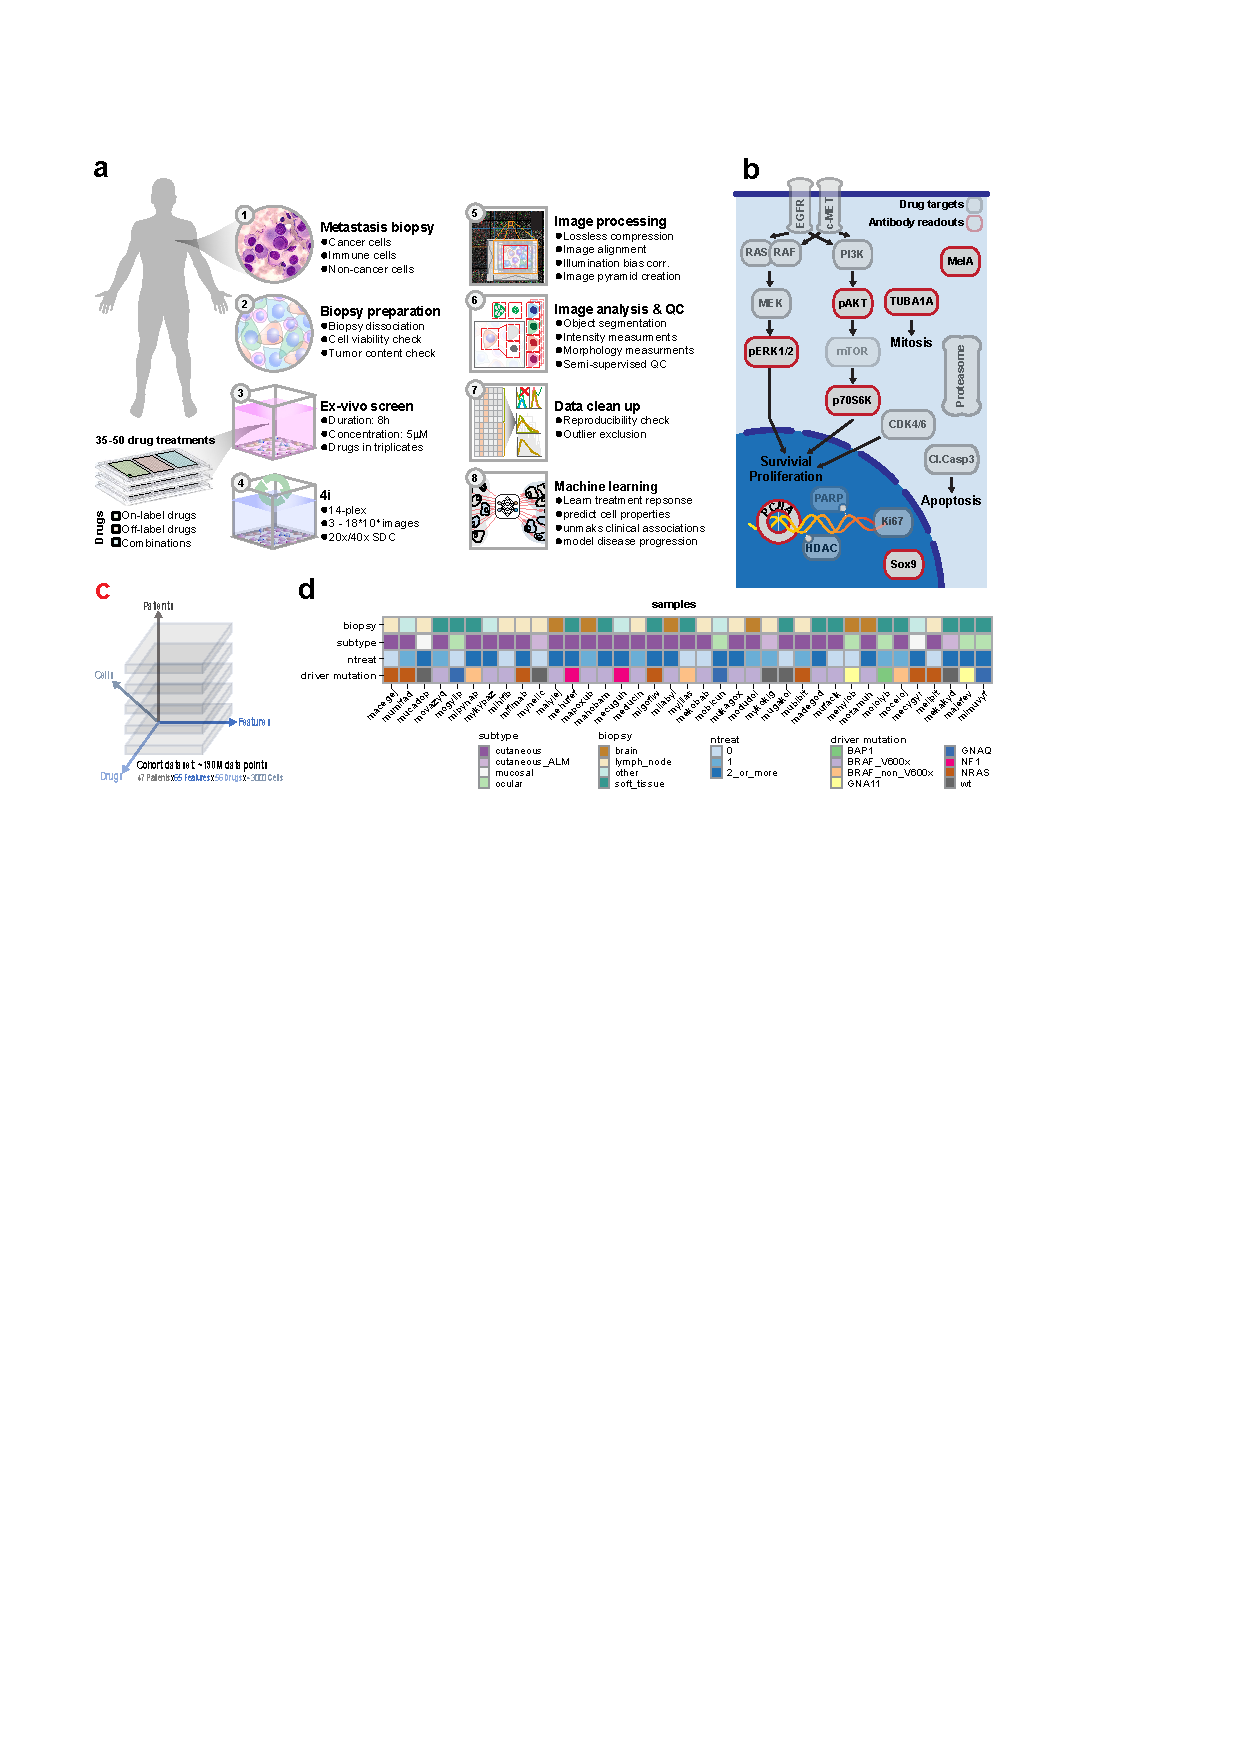
\includegraphics[width=\textwidth]{figures/cellot-cohort/overview.pdf}
  \caption{
    Predicting single-cell responses of progressed melanoma patients.
    From sample collection to machine learning to evaluation.
    a) 4i DRP pipeline for a single sample from tumor profiler.
    1-4: a tumor biopsy is taken from a cancer patient, prepared,
    exposed, in parallel, to $N$ treatments (including control).
    Cell morphology and marker intensities are imaged.
    5-6: An in house imaging processing pipeline performs cell segmentation,
    extracts marker intensity levels and morphology features.
    7: Extracted features are selected, standardized, normalized and batch corrected.
    8: Modeling and validation of single-cell responses in two settings: learning individual responses and predicting responses of \emph{incoming} samples
    b) 4i-profiled markers are selected from known key signalling pathways in cancer.
    c) In total, 47 patients are profiled, XX cellular features are extracted, XX drug responses are measured, each containing about 3000 cells. In total over 190M cells are profiled.
    d) The melanoma cohort represents a diverse, heterogenous set of samples,\
    across biopsy location, cancer subtype, number of lines of treatment, and (known) driver mutation.
  }
\end{figure*}

\subsection{Data}
% TODO: describe cohort composition

\paragraph{Normalization}
The extracted features are then further normalized and processed to remove batch effects and standardize the range of values. First, wells with an abnormally low number of cells (50) are considered low-quality and are removed. The range of feature values are then standardized with a quantile rescaling computed on the individual morphological features and the joint intensity features. After, the level of background light intensity for each plate is computed and removed. A secondary control that … is included in each plate. In order to standardize the intensity level of the protein markers across plates, the intensity features of the secondary control are computed and cells on the plate with intensity features below the 75th quantile are clipped. An additional quality control is then applied to cells that are inflated for no marker intensity. Cells are removed in which four or more intensity features are measured as zero. Finally, a variance stabilizing monotonic log + 1 transform is performed to mitigate the influence of any extreme outliers in both the morphological and intensity features.

% TODO: describe replicates, normalization validation

\subsection{Model training, IID}
Heterogeneous single-cell perturbation responses are computed for each treatment using CellOT [CITE]. Optimal transport is a rich field of mathematics that describes how to align probability distributions according to a principle of minimum action. In this case, we are unable to observe the state of a cell before and after treatment, thus we rely on the optimal transport map to inform us what the individual cellular responses were that transformed the set of observed untreated (control) cells into the set of observed treated cells. CellOT utilizes neural optimal transport theory to learn a neural-network parameterization of this optimal transport map, allowing us to make predictions on cells that are not available at training time.

We demonstrate the ability of CellOT to learn the responses tumor cells take to each treatment, individually for each patient. The cells of each sample are split into a 75/10/15 train/valid/test split, computed individually for each treatment. We train the model using cells from the train split, perform validation and any intermediate analyses on the valid split, and only communicate results using predictions made on the test split. Since all splits are sampled from the same sample in an independent and identically distributed (IID) manner, we refer to this setting as the IID setting.

We use the default architecture and hyperparameter choices of CellOT, networks have a width of 64 and depth of 4, convexity on the transporting potential is enforced with a regularization term with equal weight to the loss, we use the Adam optimizer [cite] with a learning rate of 1e-4, a beta of (0.5, 0.9), an inner loop of 10 steps and perform the outer loop for 100000 steps, a number picked as a conservative estimate to ensure convergence. Since these networks are relatively small, they can be comfortably trained on CPUs and are trained in less than 2 hours. 

\subsection{Model training, OOD}
In this experiment, we demonstrate how we can learn to generalize a set of observed treatment responses to incoming, unseen samples. To do so,  for each sample, for each treatment, we train a CellOT model on the composite set of all other samples and then predict the responses of the held out sample. This is often referred to as a hold-one-out experiment, and is also an example of an on out-of-distribution (OOD) prediction task, since the distribution of cellular states in the training set (the cohort) is different from the test set (the holdout sample). We train all models as we had done in the IID experiments, using the same training splits and evaluate using the same set of test cells to keep the experiments comparable.  We furthermore introduce an additional evaluation metric by computing the distance of the CellOT predictions made in the IID and OOD setting.

\subsection{Conditional CellOT}
When training models to handle the prediction of responses across a cohort of samples, as is done in the OOD setting, meta information not necessarily contained in the cell feature space may be informative towards the nature of cellular responses. For instance, some targeted therapies are designed to treat patients with a specific driver mutation and thus we can expect that patients with these driver mutations may respond differently than those without. While the base model of CellOT is only able to make predictions from cellular features, [Bunne et al] described an approach to condition predictions on meta information.

We train a conditional CellOT model using one-hot encodings of both the individual’s known driver mutation and the number of lines of treatment applied. The former is included to handle the differential responses of targeted therapies while the latter is included since lines of treatment indicate a degree of the acquired immunity of tumor cells.

\subsection{Comparisons}
We compare the performance of CellOT to several baselines, including two auto-encoder baselines. scGen [cite] and the conditional auto-encoder (cAE) [CITE] and a simple baseline that predicts responses as the average between the two conditions. While CellOT applies treatment effects directly on the observed cell features themselves, scGen and cAE both rely on auto-encoders to learn compressed representations of cells and apply treatment effects on these representations. For each we use a two layer encoder and decoders with a width of 32 and a bottleneck width of 8. We train with the same data splits and using the default Adam parameters for a total of 100000 iterations.
